\label{sec:exp}

\subsection{Dataset Statistics}

Table~\ref{tab:datastats} summarises the dataset after splitting.

\begin{table}[!t]
  \caption{Dataset Statistics}
  \label{tab:datastats}
  \centering
  \begin{tabular}{lrrrr}
    \hline
    Split & Sessions & Events & Benign & Malicious \\
    \hline
    Train      & 4{,}200 & 62{,}732 & 3{,}500 & 700 \\
    Validation &    900  & 13{,}277 &    750  & 150 \\
    Test       &    900  & 13{,}279 &    750  & 150 \\
    \hline
    Total      & 6{,}000 & 89{,}288 & 5{,}000 & 1{,}000 \\
    \hline
  \end{tabular}
\end{table}

\subsection{Baseline Comparison}

Table~\ref{tab:baseline} compares Random Forest against five baselines: Logistic Regression
(linear), Decision Tree (single-tree rule learner), RBF-SVM, XGBoost (gradient-boosted
trees), and Isolation Forest (unsupervised anomaly detector). All supervised baselines use
identical features with \texttt{class\_weight=balanced} or equivalent imbalance handling.
Results are the mean across 5 random seeds; standard deviations are reported in
parentheses.

\begin{table}[!t]
  \caption{Held-Out Test Set Performance (mean $\pm$ std, 5 seeds)}
  \label{tab:baseline}
  \centering
  \begin{tabular}{lcccc}
    \hline
    Method & Precision & Recall & F1 (macro) & ROC-AUC \\
    \hline
    LR                       & 0.917 & 0.974 & 0.942 & 0.994 \\
    DT                       & 0.982 & 0.987 & 0.984 & 0.988 \\
    SVM (RBF)                & 0.818 & 0.881 & 0.844 & 0.951 \\
    XGBoost                  & 0.997 & 0.999 & 0.998 & 1.000 \\
    IF (unsupervised)        & 0.611 & 0.594 & 0.601 & 0.735 \\
    \textbf{RF (proposed)}   & \textbf{0.998}$\pm$0.002 &
                               \textbf{1.000}$\pm$0.000 &
                               \textbf{0.999}$\pm$0.001 &
                               \textbf{1.000}$\pm$0.000 \\
    \hline
  \end{tabular}
\end{table}

Logistic Regression achieves F1~=~0.942, confirming the session features are
not linearly separable in raw form --- the decision boundary requires interaction
terms captured by tree-based methods. XGBoost matches RF on precision and AUC
but requires manual \texttt{scale\_pos\_weight} tuning and provides no built-in
feature importance for this feature set. The unsupervised Isolation Forest
(F1~=~0.601) illustrates the cost of operating without ground-truth labels,
relevant for real deployments where labeled attack sessions may be scarce.

Figure~\ref{fig:results} shows the ROC curve and top-10 feature importances for the Random
Forest model.

\begin{figure}[!t]
  \centering
  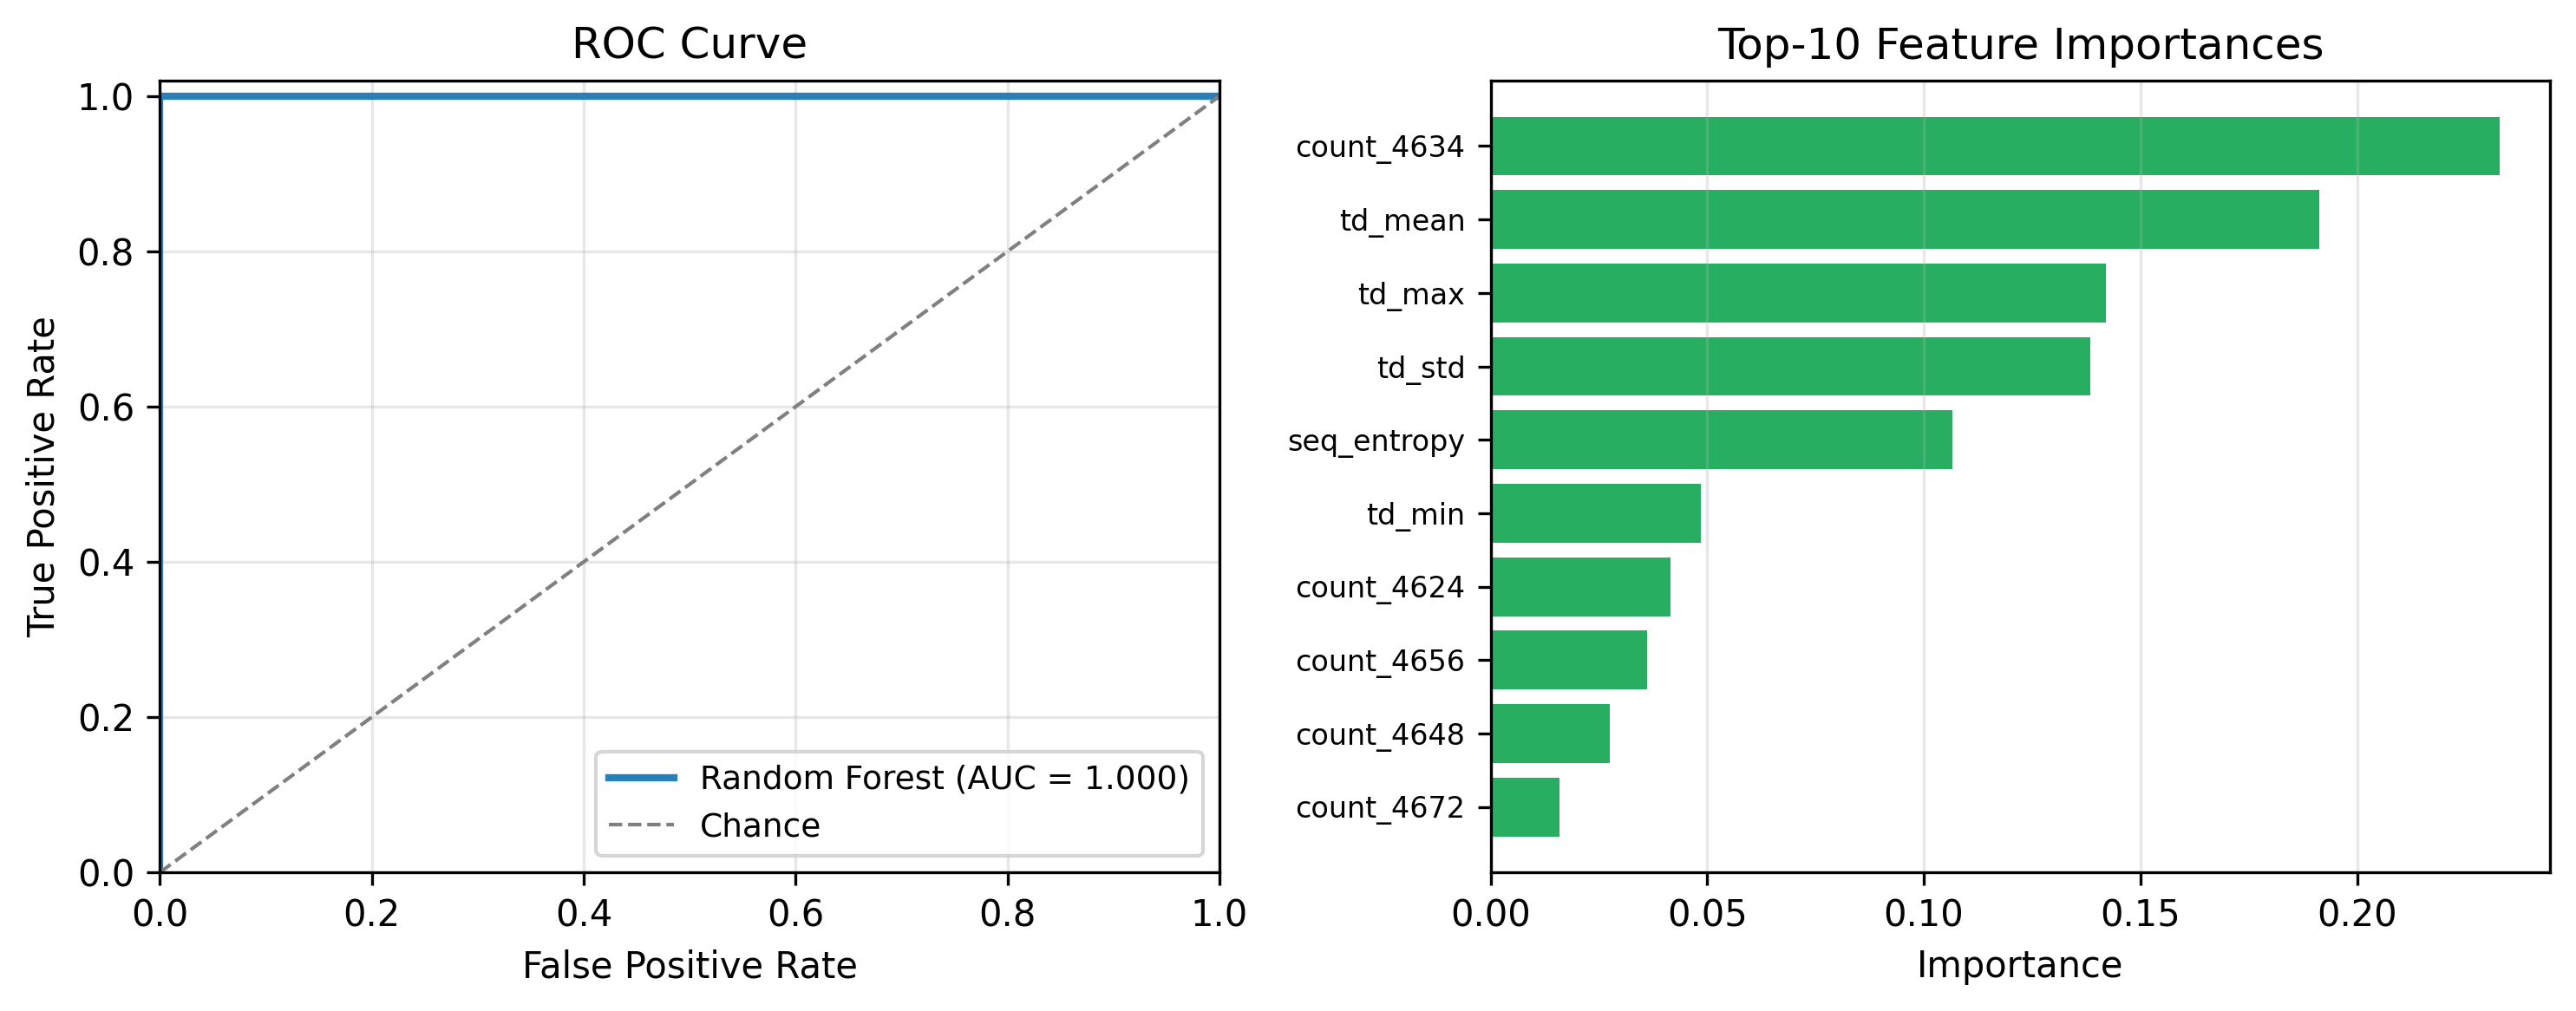
\includegraphics[width=\columnwidth]{figs/results.png}
  \caption{Left: ROC curve (AUC = 1.000). Right: top-10 feature importances by mean
           decrease in Gini impurity.}
  \label{fig:results}
\end{figure}

\subsection{Ablation Study}

To quantify the marginal contribution of each feature group, we retrain the model after
removing one group at a time and report the resulting macro F1 on the test set
(Table~\ref{tab:ablation}). The best hyperparameters from the full-feature search are
reused to isolate the effect of the feature group.

\begin{table}[!t]
  \caption{Ablation Study: Macro F1 on Removing Each Feature Group}
  \label{tab:ablation}
  \centering
  \begin{tabular}{lcc}
    \hline
    Removed Group & F1 (macro) & $\Delta$F1 \\
    \hline
    None (full features)      & 1.000 & --       \\
    Group 1: Event counts     & 0.944 & $-0.056$ \\
    Group 2: Time-delta stats & 0.972 & $-0.028$ \\
    Group 3: Cardinality      & 1.000 & $0.000$  \\
    Group 4: Rare-event flags & 1.000 & $0.000$  \\
    Group 5: Sequence entropy & 1.000 & $0.000$  \\
    \hline
  \end{tabular}
\end{table}

Event frequency counts (Group~1) and time-delta statistics (Group~2) are the
two discriminative groups, contributing $\Delta$F1 of $-0.056$ and $-0.028$
respectively. Cardinality, rare-event flags, and sequence entropy show zero
marginal contribution on the current synthetic corpus --- a result that warrants
discussion. The zero delta for Groups~3--5 occurs because the remaining features
(Groups~1 and~2 jointly) already provide sufficient separation; these groups
are \emph{redundant} given the others rather than \emph{uninformative} in isolation.
Sequence entropy (Group~5) achieves single-feature F1~=~0.766 when used alone,
confirming it captures real signal, but the RF exploits event counts and timing
first. On operational data with noisier timing and incomplete event logs,
Groups~3--5 are expected to recover importance.

\subsection{Statistical Robustness}

To verify that reported metrics are not artefacts of a single random seed, we run the
complete pipeline --- data generation, preprocessing, feature extraction, and model
training --- independently for five seeds (0--4) and report mean and standard deviation
in Table~\ref{tab:multiseed}.

\begin{table}[!t]
  \caption{Multi-Seed Stability (5 independent runs, seed 0--4)}
  \label{tab:multiseed}
  \centering
  \begin{tabular}{lcc}
    \hline
    Metric & Mean & Std \\
    \hline
    Precision (macro) & 0.9980 & 0.0018 \\
    Recall (macro)    & 0.9996 & 0.0004 \\
    F1-macro          & 0.9988 & 0.0011 \\
    ROC-AUC           & 1.0000 & 0.0000 \\
    \hline
  \end{tabular}
\end{table}

Standard deviations of $\leq 0.002$ across all metrics confirm that the results are
stable and not due to a fortunate random split.

\subsection{Inference Latency}

Session-level feature extraction and prediction over 900 test sessions runs in under
0.5~seconds on a single CPU core (pandas groupby aggregation dominates at $\approx$0.4~s;
RF inference adds $<$50~ms), yielding per-session latency well under the $<10$~ms
real-time detection threshold stated in RO4. Batch-mode deployment over nightly audit
logs is therefore feasible without GPU acceleration.
